\documentclass[paper=a4, fontsize=10pt]{scrartcl} % A4 paper and 11pt font size

\usepackage[T1]{fontenc} % Use 8-bit encoding that has 256 glyphs
\usepackage{fourier} % Use the Adobe Utopia font for the document - comment this line to return to the LaTeX default
\usepackage[english]{babel} % English language/hyphenation
\usepackage{amsmath,amsfonts,amsthm} % Math packages
\usepackage{graphicx}
\usepackage[cm]{fullpage}
\usepackage{float}
\usepackage{sectsty} % Allows customizing section commands
\allsectionsfont{\centering \normalfont\scshape} % Make all sections centered, the default font and small caps

\usepackage{fancyhdr} % Custom headers and footers
\pagestyle{fancyplain} % Makes all pages in the document conform to the custom headers and footers
\fancyhead{} % No page header - if you want one, create it in the same way as the footers below
\fancyfoot[L]{} % Empty left footer
\fancyfoot[C]{} % Empty center footer
\fancyfoot[R]{\thepage} % Page numbering for right footer
\renewcommand{\headrulewidth}{0pt} % Remove header underlines
\renewcommand{\footrulewidth}{0pt} % Remove footer underlines
\setlength{\headheight}{13.6pt} % Customize the height of the header

\numberwithin{equation}{section} % Number equations within sections (i.e. 1.1, 1.2, 2.1, 2.2 instead of 1, 2, 3, 4)
\numberwithin{figure}{section} % Number figures within sections (i.e. 1.1, 1.2, 2.1, 2.2 instead of 1, 2, 3, 4)
\numberwithin{table}{section} % Number tables within sections (i.e. 1.1, 1.2, 2.1, 2.2 instead of 1, 2, 3, 4)

\setlength\parindent{0pt} % Removes all indentation from paragraphs - comment this line for an assignment with lots of text

%----------------------------------------------------------------------------------------
%	TITLE SECTION
%----------------------------------------------------------------------------------------

\newcommand{\horrule}[1]{\rule{\linewidth}{#1}} % Create horizontal rule command with 1 argument of height

\newtoks\rowvectoks
\newcommand{\rowvec}[2]{%
  \rowvectoks={#2}\count255=#1\relax
  \advance\count255 by -1
  \rowvecnexta}
\newcommand{\rowvecnexta}{%
  \ifnum\count255>0
    \expandafter\rowvecnextb
  \else
    \begin{pmatrix}\the\rowvectoks\end{pmatrix}
  \fi}
\newcommand\rowvecnextb[1]{%
    \rowvectoks=\expandafter{\the\rowvectoks&#1}%
    \advance\count255 by -1
    \rowvecnexta}

\title{	
\normalfont \normalsize 
\textsc{Radboud University Nijmegen}  % Your university, school and/or department name(s)
\horrule{0.5pt} \\[0.3cm] % Thin top horizontal rule
\huge Statistical Machine Learning \\ Assignment 4 \\ % The assignment title
\horrule{2pt}  % Thick bottom horizontal rule
}

\author{Steven Reitsma \\ (s4132343)} % Your name

\date{\normalsize\today} % Today's date or a custom date

\begin{document}

\maketitle % Print the title

\section{EM and doping}
\subsection{Visualizing the data}
Plotting $x_1$ on the x-axis, $x_2$ on the y-axis, and the sum of $x_3$ and $x_4$ as the color gives the plot as shown in Figure \ref{visualization}. We can definitely see some structure in the data, annotated in Figure \ref{visualization_annotated}. If we plot the variables in 3d-space, with $x_1$ on the x-axis, $x_2$ on the y-axis, $x_3$ on the z-axis and $x_4$ as color, we can see that there is a cloud of points that forms a perpendicular plane to the other cloud of points. This is the same cloud of points that is visible in the 2d-plot as the purple class (see Figure \ref{visualization_annotated}). The 3d-visualization can be shown by running the \verb|exercise_11_3d.py| file (requires \verb|matplotlib| and \verb|mpltools|).

\begin{figure}[h!]
	\centering
	\includegraphics[width=0.75\textwidth]{exercise_11.pdf}.
	\caption{Plot of the data set with $x_1$ on the x-axis, $x_2$ on the y-axis, and $x_3 + x_4$ as the color.}
	\label{visualization}
\end{figure}

\begin{figure}[h!]
	\centering
	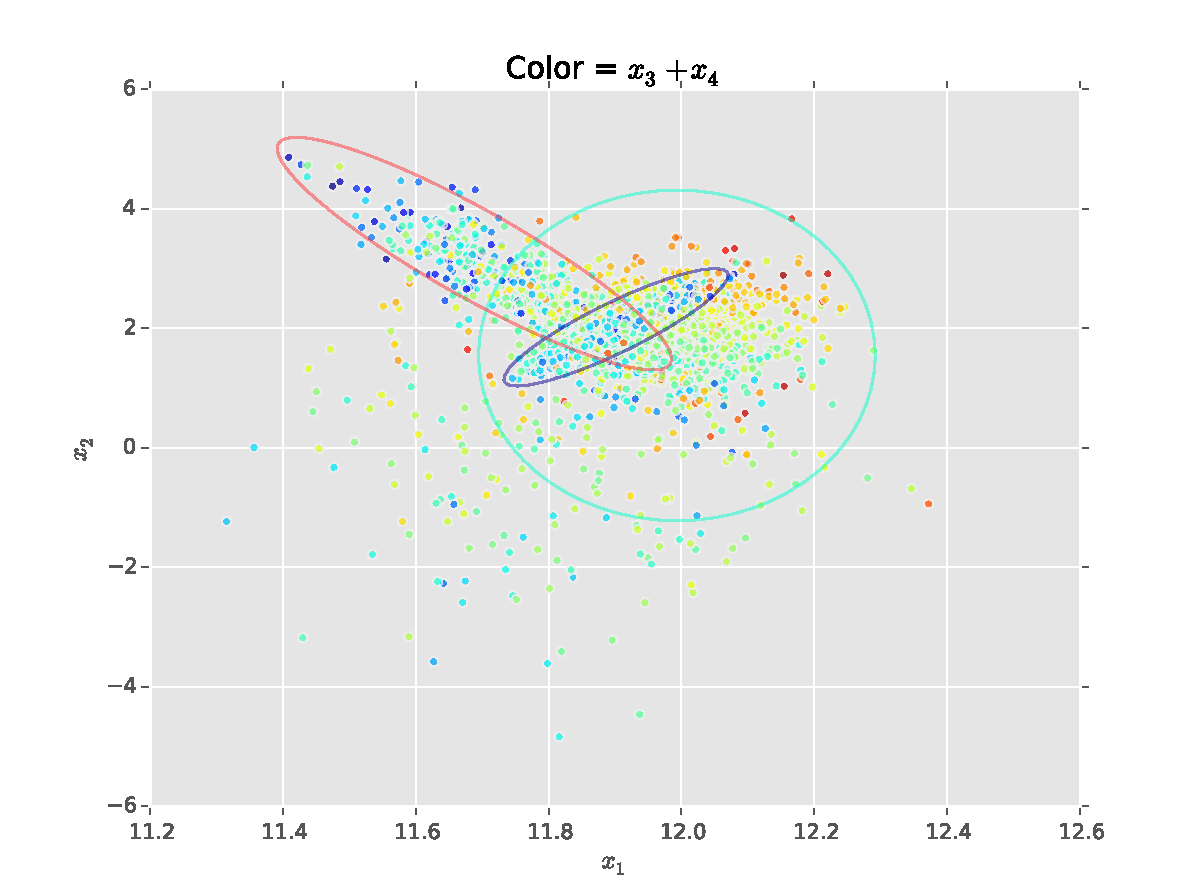
\includegraphics[width=\textwidth]{exercise_11_annotated.pdf}.
	\caption{The different classes that can be observed in the data. The cyan class is the largest one, where there is no correlation between $x_1$ and $x_2$. The purple class has a positive correlation between $x_1$ and $x_2$, while the orange class has a negative correlation between $x_1$ and $x_2$. The purple and cyan classes can be distinguished easily using $x_3$ and $x_4$. Seperating the orange class seems harder.}
	\label{visualization_annotated}
\end{figure}

\end{document}